\subsection{Editor Extension Components}

This section will describe the most relevant components, libraries or widgets for \acrshort{emf} in the \gls{cloud}, which can be used to create editor extensions.


\subsubsection{Sprotty}
Eclipse Sprotty is a library to render diagrams in web browsers.
It uses Typescript, CSS and svg.
Sprotty can animate diagram changes.
The architecture is made with \gls{LSP} in mind, and supports having diagram data sent from a backend.
The library is configurable using dependency injection, and allows for adding custom nodes, edges and behaviors.
It also provides ``glue code'' for easy integration with \gls{LSP}, \gls{Theia} and \gls{ELK}.~\cite{smithEclipseSprotty2018}
An example of a sprotty diagram is shown in \cref{fig:sprotty-example}.

The library is mainly developed by TypeFox and EclipseSource, and managed by the Eclipse Foundation.~\cite{eclipsefoundationEclipseSprotty}

\begin{figure}[htbp]  % order of priority: h here, t top, b bottom, p page
  \centering
  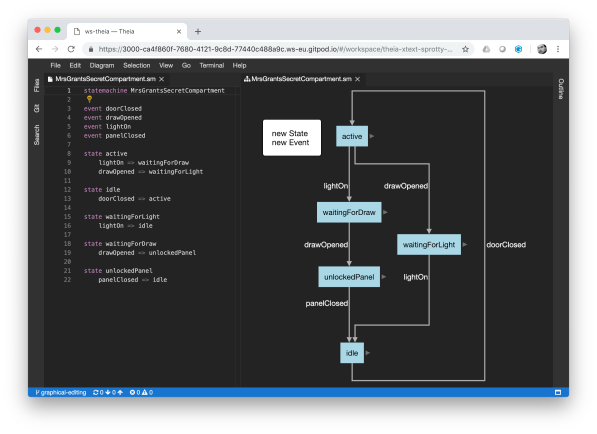
\includegraphics[width=.5\textwidth]{figures/sprotty-example.png}
  \caption[Sprotty Example]{This is a screenshot of Theia with a Sprotty diagram on the right side.~\cite{eclipsefoundationEclipseSprotty2020}}\label{fig:sprotty-example}
\end{figure}

% TODO: write
% What is it?
% Who made it?


\subsubsection{EMF.Cloud --- Theia Tree Editor}
% TODO: write
% What is it?
% Who made it?

% JSON-Forms ?
% Model Server?
% Eclipse Edit?
% 